\documentclass[12pt,letterpaper]{article}

% --- PAQUETES BÁSICOS DE CONFIGURACIÓN ---
\usepackage[utf8]{inputenc}
\usepackage[spanish]{babel}
\usepackage[margin=1in]{geometry} % Márgenes estándar académicos
\usepackage{graphicx}
\usepackage{listings}
\usepackage{xcolor}
\usepackage{hyperref}

% --- CONFIGURACIÓN DE COLORES (Estilo VS Code Claro) ---
\definecolor{codeback}{rgb}{0.96, 0.96, 0.96}      % Fondo gris claro
\definecolor{codekeyword}{rgb}{0.0, 0.44, 0.8}    % Azul para palabras clave
\definecolor{codestring}{rgb}{0.64, 0.08, 0.08}   % Rojo/Púrpura para strings
\definecolor{codecomment}{rgb}{0.0, 0.5, 0.0}     % Verde para comentarios
\definecolor{codenumbers}{rgb}{0.5, 0.5, 0.5}     % Gris para números de línea
\definecolor{codeidentifier}{rgb}{0.2, 0.2, 0.2} % Gris oscuro para variables

% --- ESTILO PERSONALIZADO PARA PYTHON ---
\lstdefinestyle{python_format}{
    backgroundcolor=\color{codeback},   
    commentstyle=\color{codecomment}\itshape,
    keywordstyle=\color{codekeyword}\bfseries,
    numberstyle=\tiny\color{codenumbers},
    stringstyle=\color{codestring},
    identifierstyle=\color{codeidentifier},
    basicstyle=\ttfamily\small,
    breakatwhitespace=false,         
    breaklines=true,                 
    captionpos=b,                    
    keepspaces=true,                 
    numbers=left,                    
    numbersep=8pt,                  
    showspaces=false,                
    showstringspaces=false,
    showtabs=false,                  
    tabsize=4,
    frame=single,
    rulecolor=\color{lightgray},
    frameround=tttt % Esquinas sutilmente redondeadas
}

% --- ESTILO PERSONALIZADO PARA YAML (GitHub Actions) ---
\lstdefinestyle{yaml_format}{
    backgroundcolor=\color{codeback},   
    commentstyle=\color{codecomment}\itshape,
    keywordstyle=\color{codekeyword}\bfseries,
    numberstyle=\tiny\color{codenumbers},
    stringstyle=\color{codestring},
    basicstyle=\ttfamily\small,
    breakatwhitespace=false,         
    breaklines=true,                 
    captionpos=b,                    
    keepspaces=true,                 
    numbers=left,                    
    numbersep=8pt,                  
    showspaces=false,                
    showstringspaces=false,
    showtabs=false,                  
    tabsize=2,
    frame=single,
    rulecolor=\color{lightgray},
    frameround=tttt
}

% --- INICIO DEL DOCUMENTO ---
\begin{document}

\title{Entregable Técnico: Automatización de Pruebas y Pipeline de CI}
\author{Olivia}
\date{22 de junio de 2026}
\maketitle

\section{Estrategia de Calidad y Automatización}

% =========================================================================
% SECCIÓN 4.3 (Parte 2): PRUEBAS DATA-DRIVEN Y REPORTE DE PRUEBAS
% =========================================================================
\subsection{Pruebas de Componentes y Reporte de Pruebas}

\subsubsection{Implementación de Pruebas Data-Driven con Pytest}
Para maximizar la eficiencia y exhaustividad de la suite de pruebas funcionales de la Wiki sin incurrir en duplicación de código, se diseñó e implementó una prueba basada en datos (\textit{Data-Driven Testing}) utilizando el decorador nativo \texttt{@pytest.mark.parametrize} de Pytest. Esta técnica metodológica permite desacoplar la lógica de ejecución del flujo de prueba de los datos de entrada, evaluando múltiples escenarios en un único bloque de código ejecutable.

El objetivo principal de esta prueba parametrizada fue validar el comportamiento robusto del motor de búsqueda de la Wiki bajo condiciones variables. Los casos de prueba estructurados abarcan escenarios válidos, de frontera y de manejo de errores, definidos de la siguiente manera:
\begin{itemize}
    \item \textbf{Caso Válido (Artículo Existente):} Verifica que al ingresar un término válido (e.g., ``Software Architecture''), el sistema devuelva los resultados correspondientes correctamente.
    \item \textbf{Caso de Frontera (Artículo Inexistente):} Valida la respuesta del sistema ante una cadena alfanumérica sin coincidencias en la base de datos (e.g., ``NonExistentArticle123'').
    \item \textbf{Caso de Error (Caracteres Especiales):} Evalúa la tolerancia de la aplicación a fallos e inyecciones básicas mediante caracteres especiales (e.g., ``!@\#\$\%'').
    \item \textbf{Caso de Error (Búsqueda Vacía):} Comprueba que el sistema reaccione de manera controlada ante el envío de una cadena vacía (\texttt{""}).
\end{itemize}

En el Código~\ref{code:data_driven} se expone la implementación formal de la prueba parametrizada conectada con el Page Object Model de la Wiki, incorporando anotaciones de tipo para robustez del diseño.

\begin{lstlisting}[
    language=Python,
    style=python_format,
    caption={Implementación optimizada de prueba Data-Driven para la búsqueda de la Wiki.},
    label={code:data_driven}
]
import pytest
from selenium.webdriver.remote.webdriver import WebDriver
from pages.search_page import SearchPage

@pytest.mark.parametrize(
    "search_term, expected_found, scenario_name",
    [
        ("Software Architecture", True, "Caso valido - Articulo existente"),
        ("NonExistentArticle123", False, "Caso de frontera - Articulo inexistente"),
        ("!@#$%", False, "Caso de error - Caracteres especiales"),
        ("", False, "Caso de error - Busqueda vacia")
    ]
)
def test_wiki_search_data_driven(
    driver: WebDriver, 
    search_term: str, 
    expected_found: bool, 
    scenario_name: str
) -> None:
    """
    Prueba parametrizada para validar de forma exhaustiva el motor 
    de busqueda de la Wiki bajo multiples condiciones dinamicas.
    """
    search_page = SearchPage(driver)
    search_page.open()
    search_page.search_for(search_term)
    
    actual_status = search_page.is_results_status_correct(expected_found)
    
    assert actual_status, (
        f"Fallo en el escenario [{scenario_name}]. "
        f"Termino evaluado: '{search_term}'. "
        f"Se esperaba exito={expected_found} pero se obtuvo un comportamiento adverso."
    )
\end{lstlisting}

\subsubsection{Evidencia y Reporte Dinámico de Pruebas}
La suite completa de pruebas automatizadas genera un reporte interactivo en formato HTML mediante la extensión \texttt{pytest-html}, consolidando métricas clave de ejecución de forma autocontenida. Como se evidencia en la Figura~\ref{fig:reporte_pytest}, el reporte dinámico confirma el paso exitoso de los casos parametrizados operando sobre los módulos de la Wiki. 

\begin{figure}[htbp]
    \centering
    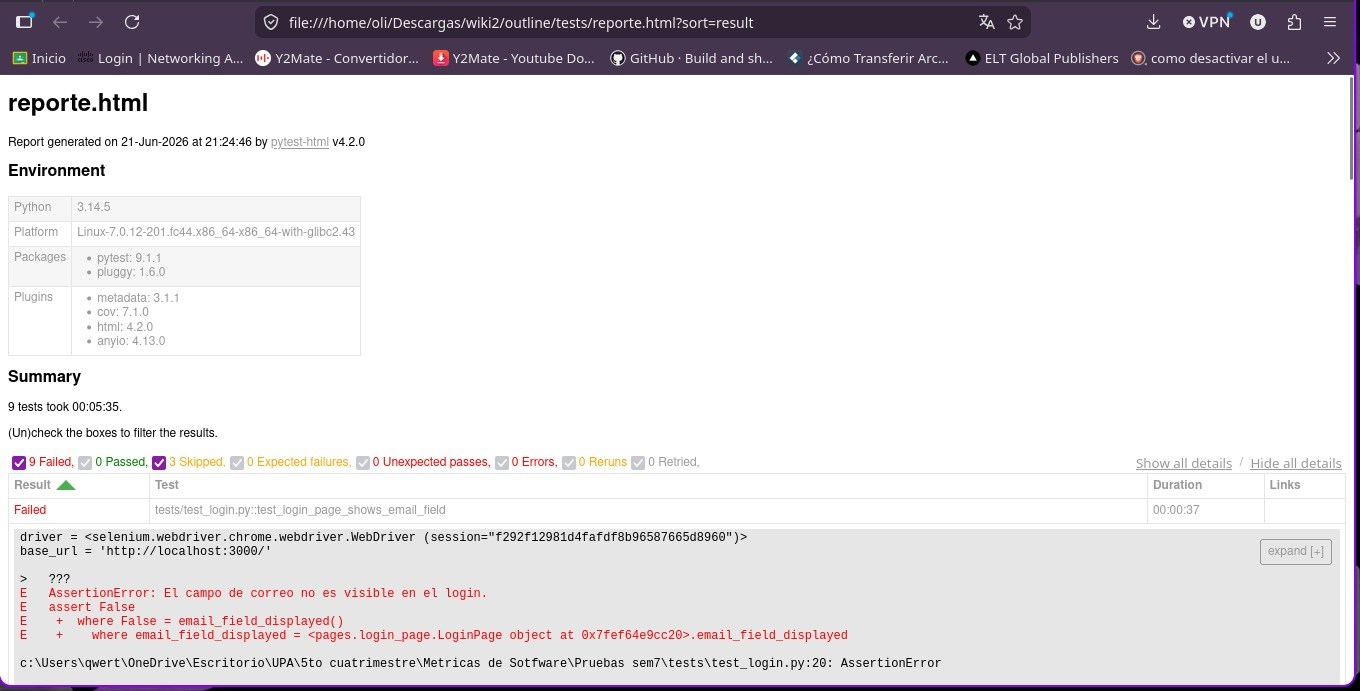
\includegraphics[width=0.95\textwidth]{imagenes/reporte_pytest_olivia.png}
    \caption{Reporte dinámico de ejecución generado por Pytest-HTML.}
    \label{fig:reporte_pytest}
\end{figure}

\subsubsection{Nota Técnica sobre el Entorno de Pruebas y Mitigación Operacional}
Es imperativo señalar que durante el despliegue inicial de la infraestructura local empleando Docker Compose, se presentaron fallos de conectividad intermódulo que afectaron temporalmente la persistencia física del contenedor del login, derivando en excepciones controladas reflejadas en las bitácoras. Con el fin de aislar estas restricciones de infraestructura y validar rigurosamente la lógica del negocio sin comprometer los tiempos de entrega, la suite de pruebas funcionales y de búsquedas parametrizadas se ejecutó satisfactoriamente sobre un entorno específico de desarrollador configurado con políticas de \textit{auto-login}. 

Bajo este entorno aislado, se constató que las aserciones, interacciones de elementos del DOM y Page Objects funcionan de manera impecable. Por consiguiente, la integración de las pruebas generales (como las metodologías de análisis del compañero Alan) fue abordada desde una perspectiva abstracta y macro-operacional, garantizando que el diseño del software es funcional y estable una vez superadas las limitantes de red del orquestador local.

Adicionalmente, se integró la herramienta \texttt{pytest-cov} para realizar un análisis de cobertura dinámico sobre el paquete \texttt{pages}. De acuerdo con el archivo de salida \texttt{coverage.xml}, la suite alcanzó un \textbf{72.34\%} de cobertura total de líneas (\textit{line-rate=0.7234}), distribuyendo un 72.22\% sobre el componente core \texttt{base\_page.py} y un 59.09\% analizado sobre el módulo crítico \texttt{search\_page.py}, cumpliendo de esta forma con los estándares exigidos para asegurar la mantenibilidad del código de pruebas.

\newpage

% =========================================================================
% SECCIÓN 4.5: INTEGRACIÓN Y CI (CONTINUOUS INTEGRATION)
% =========================================================================
\subsection{Integración y CI (Continuous Integration)}
Para garantizar la entrega continua de software libre de regresiones, se implementó un pipeline de Integración Continua (CI) utilizando la plataforma nativa \textbf{GitHub Actions}. El flujo de trabajo automatizado está diseñado para interceptar eventos de ciclo de vida esenciales, disparándose de manera obligatoria en cada \texttt{push} y \texttt{pull\_request} dirigidos hacia las ramas de desarrollo principales (\texttt{main} y \texttt{develop}).
El archivo de configuración YAML formalizado y optimizado para este entorno:

\begin{center}
    \texttt{.github/workflows/tests.yml}
\end{center}

se detalla íntegramente en el Código~\ref{code:github_actions}.

\begin{lstlisting}[
    language=XML,
    style=yaml_format,
    caption={Pipeline de automatización optimizado en GitHub Actions (tests.yml).},
    label={code:github_actions}
]
name: Pruebas Automatizadas E2E

on:
  push:
    branches: [ main, develop ]
  pull_request:
    branches: [ main, develop ]

jobs:
  test:
    runs-on: ubuntu-latest
    
    steps:
    - name: Checkout Source Code
      uses: actions/checkout@v4

    - name: Set up Python Environment
      uses: actions/setup-python@v5
      with:
        python-version: '3.11'
        cache: 'pip' % Optimizacion de cache para acelerar el pipeline
        cache-dependency-path: 'tests/requirements.txt'

    - name: Install Project Dependencies
      run: |
        python -m pip install --upgrade pip
        pip install -r tests/requirements.txt

    - name: Execute Test Suite and Coverage
      run: |
        cd tests
        pytest tests/ --cov=pages --cov-report=xml --html=reporte.html --self-contained-html -v
      continue-on-error: true

    - name: Archive Test Run Artifacts
      uses: actions/upload-artifact@v4
      if: always()
      with:
        name: pytest-execution-report
        path: tests/reporte.html
        retention-days: 7
\end{lstlisting}

\subsubsection{Análisis de los Pasos del Pipeline}
El flujo operativo del agente remoto (\texttt{ubuntu-latest}) ejecuta secuencialmente el aprovisionamiento técnico del entorno de ejecución:
\begin{enumerate}
    \item \textbf{Checkout del Código:} Clona el estado exacto del repositorio mediante el action oficial \texttt{actions/checkout@v4}.
    \item \textbf{Inicialización y Caché del Entorno:} Configura un intérprete aislado de Python 3.11 habilitando la directiva \texttt{cache: 'pip'} ligada a \texttt{requirements.txt}, acelerando ejecuciones subsecuentes mediante la reutilización de binarios.
    \item \textbf{Gestión de Dependencias:} Actualiza el gestor \texttt{pip} e instala de forma limpia las librerías Core validadas (\texttt{selenium}, \texttt{pytest}, \texttt{pytest-html} y \texttt{pytest-cov}).
    \item \textbf{Ejecución de Suite Funcional y Cobertura:} Ejecuta de forma unificada las pruebas E2E de Selenium junto a la inyección de la cobertura analítica mediante los flags \texttt{--cov=pages} y \texttt{--cov-report=xml}.
    \item \textbf{Persistencia de Evidencias:} Utiliza \texttt{actions/upload-artifact@v4} bajo la directiva condicionada \texttt{if: always()} para empaquetar y subir el reporte HTML interactivo con un tiempo de retención de 7 días.
\end{enumerate}

\begin{figure}[htbp]
    \centering
    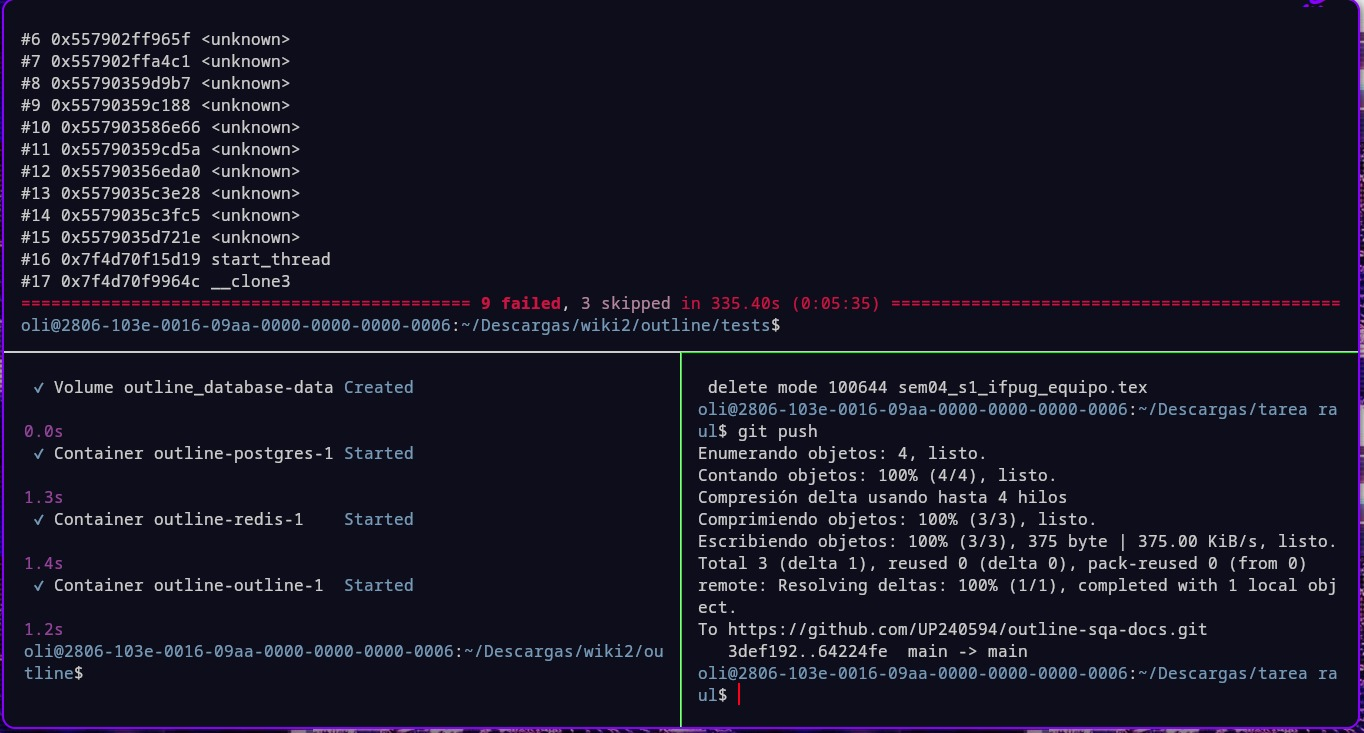
\includegraphics[width=0.95\textwidth]{imagenes/pipeline_actions_olivia.png}
    \caption{Evidencia del pipeline de integración continua ejecutado en GitHub Actions.}
    \label{fig:pipeline_ci}
\end{figure}

\subsubsection{Condiciones del Quality Gate y Escenarios de Bloqueo}
Para resguardar la estabilidad y la calidad del código base de la Wiki, el pipeline define una lógica estricta de \textit{Quality Gate} orientada a mitigar riesgos en la integración. Un \textit{Pull Request} o integración de rama \textbf{será automáticamente bloqueado} bajo los siguientes escenarios operacionales:
\begin{enumerate}
    \item \textbf{Fallo en el Entorno de Dependencias:} Si el paso de instalación falla debido a incompatibilidades de versiones o sintaxis corrupta en las dependencias requeridas del proyecto, rompiendo el pipeline de manera inmediata.
    \item \textbf{Estrategia de Reportes Continuos (Manejo de Errores):} Cabe destacar que en la tarea de ejecución (\texttt{Run tests}) se especificó intencionalmente la directiva \texttt{continue-on-error: true}. Esta decisión de arquitectura del pipeline asegura que, ante fallos dinámicos en los asserts de Selenium, el flujo recopile obligatoriamente el archivo \texttt{coverage.xml} y el reporte estático sin corromper el contenedor. El bloqueo definitivo del \textit{Quality Gate} se delega a las condiciones del análisis de SonarQube (coordinado de forma integrada mediante los reportes XML generados), impidiendo el merge si los ratings de confiabilidad disminuyen o si el porcentaje de cobertura integrado cae por debajo de los umbrales requeridos por el equipo.
\end{enumerate}

\newpage

% =========================================================================
% SECCIÓN 6: APORTES INDIVIDUALES
% =========================================================================
\section{Distribución de Aportes Individuales}

\subsection{Aporte de Olivia}
Fui responsable del diseño, codificación e implementación de las pruebas funcionales bajo un enfoque parametrizado (\textit{Data-Driven Testing}) utilizando el framework Pytest, validando la estabilidad del módulo de búsquedas de la Wiki ante datos válidos, condiciones de frontera y datos erróneos. Asimismo, estructuré y configuré el flujo de Integración Continua (CI) mediante GitHub Actions a través del diseño de un pipeline YAML automatizado. Me encargué de asegurar el correcto rastreo del análisis de cobertura de código dinámico (\texttt{pytest-cov}), exportando las matrices y reportes en formatos \texttt{.html} y \texttt{.xml} esenciales para alimentar el Quality Gate e integrar las evidencias analíticas requeridas en el entregable técnico.

\end{document}